\documentclass[11pt]{standalone}

\usepackage{tikz}
\usetikzlibrary{arrows,shapes}

\begin{document}

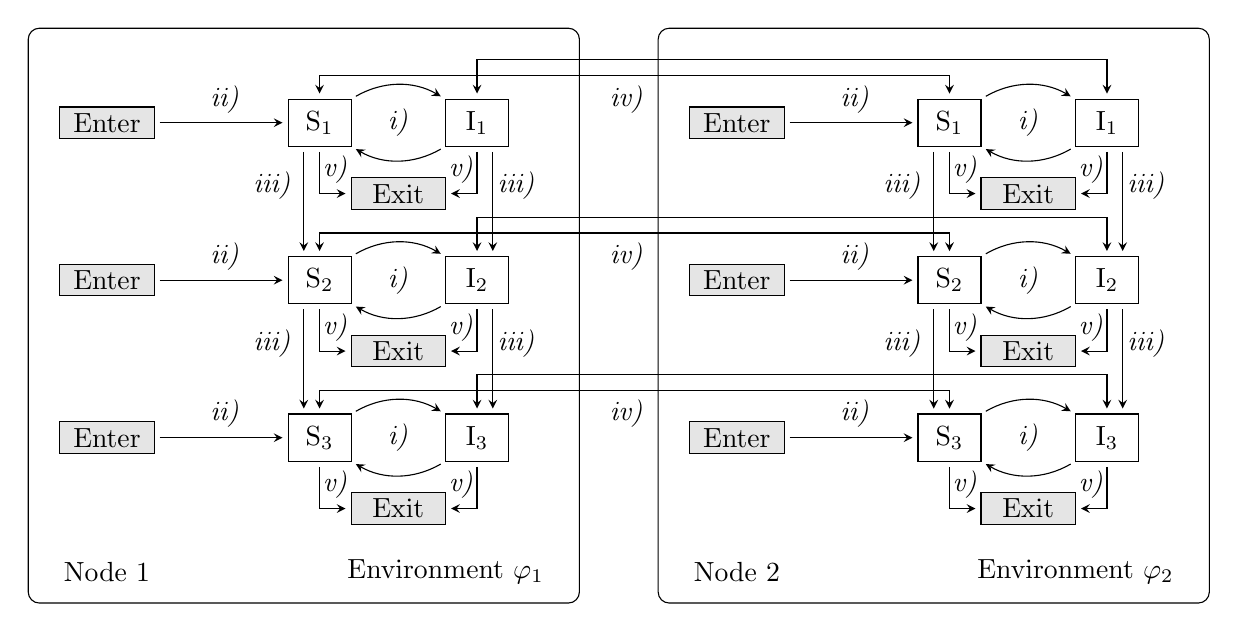
\begin{tikzpicture}[node distance=1ex]
  \draw[rounded corners] (0,-0.8) rectangle (7,6.5);
  \draw[rounded corners] (8,-0.8) rectangle (15,6.5);

  \node at (1,-0.4) {Node 1};
  \node at (9,-0.4) {Node 2};

  \node[align=center] at (5.3,-0.4) {Environment $\varphi_1$};
  \node[align=center] at (13.3,-0.4) {Environment $\varphi_2$};

  \draw [fill=black!10] (0.4,5.1) rectangle (1.6,5.5);
  \node at (1,5.3) {Enter};
  \draw [fill=black!10] (8.4,5.1) rectangle (9.6,5.5);
  \node at (9,5.3) {Enter};

  \node at (2.5,5.6) {\textit{ii)}};
  \draw[>=stealth,shorten <=2pt, shorten >=2pt,->]
  (1.6,5.3) to (3.3,5.3);
  \node at (10.5,5.6) {\textit{ii)}};
  \draw[>=stealth,shorten <=2pt, shorten >=2pt,->]
  (9.6,5.3) to (11.3,5.3);

  \draw [fill=black!10] (4.1,4.2) rectangle (5.3,4.6);
  \node at (4.7,4.4) {Exit};
  \draw [fill=black!10] (12.1,4.2) rectangle (13.3,4.6);
  \node at (12.7,4.4) {Exit};

  %% Internal transfer events
  \draw[>=stealth,shorten <=2pt, shorten >=2pt,->]
  (3.5,5) to (3.5,3.6);
  \draw[>=stealth,shorten <=2pt, shorten >=2pt,->]
  (11.5,5) to (11.5,3.6);
  \node at (3.1,4.5) {\textit{iii)}};
  \node at (11.1,4.5) {\textit{iii)}};

  \draw[>=stealth,shorten <=2pt, shorten >=2pt,->]
  (5.9,5) to (5.9,3.6);
  \draw[>=stealth,shorten <=2pt, shorten >=2pt,->]
  (13.9,5) to (13.9,3.6);
  \node at (6.2,4.5) {\textit{iii)}};
  \node at (14.2,4.5) {\textit{iii)}};

  \draw[>=stealth,shorten <=2pt, shorten >=2pt,->]
  (3.5,3) to (3.5,1.6);
  \draw[>=stealth,shorten <=2pt, shorten >=2pt,->]
  (11.5,3) to (11.5,1.6);
  \node at (3.1,2.5) {\textit{iii)}};
  \node at (11.1,2.5) {\textit{iii)}};

  \draw[>=stealth,shorten <=2pt, shorten >=2pt,->]
  (5.9,3) to (5.9,1.6);
  \draw[>=stealth,shorten <=2pt, shorten >=2pt,->]
  (13.9,3) to (13.9,1.6);
  \node at (6.2,2.5) {\textit{iii)}};
  \node at (14.2,2.5) {\textit{iii)}};

  %% External transfer events
  \draw[>=stealth,shorten <=2pt, shorten >=2pt,<->]
  (3.7,5.6) to (3.7,5.9) to (11.7,5.9) to (11.7,5.6);
  \draw[>=stealth,shorten <=2pt, shorten >=2pt,<->]
  (5.7,5.6) to (5.7,6.1) to (13.7,6.1) to (13.7,5.6);
  \node at (7.6,5.6) {\textit{iv)}};

  \draw[>=stealth,shorten <=2pt, shorten >=2pt,<->]
  (3.7,3.6) to (3.7,3.9) to (11.7,3.9) to (11.7,3.6);
  \draw[>=stealth,shorten <=2pt, shorten >=2pt,<->]
  (5.7,3.6) to (5.7,4.1) to (13.7,4.1) to (13.7,3.6);
  \node at (7.6,3.6) {\textit{iv)}};

  \draw[>=stealth,shorten <=2pt, shorten >=2pt,<->]
  (3.7,1.6) to (3.7,1.9) to (11.7,1.9) to (11.7,1.6);
  \draw[>=stealth,shorten <=2pt, shorten >=2pt,<->]
  (5.7,1.6) to (5.7,2.1) to (13.7,2.1) to (13.7,1.6);
  \node at (7.6,1.6) {\textit{iv)}};

  %% Exit events
  \draw[>=stealth,shorten <=2pt, shorten >=2pt,->]
  (3.7,5) to (3.7,4.4) to (4.1,4.4);
  \node at (3.9,4.7) {\textit{v)}};
  \draw[>=stealth,shorten <=2pt, shorten >=2pt,->]
  (5.7,5) to (5.7,4.4) to (5.3,4.4);
  \node at (5.5,4.7) {\textit{v)}};

  \draw[>=stealth,shorten <=2pt, shorten >=2pt,->]
  (11.7,5) to (11.7,4.4) to (12.1,4.4);
  \node at (11.9,4.7) {\textit{v)}};
  \draw[>=stealth,shorten <=2pt, shorten >=2pt,->]
  (13.7,5) to (13.7,4.4) to (13.3,4.4);
  \node at (13.5,4.7) {\textit{v)}};

  \draw[>=stealth,shorten <=2pt, shorten >=2pt,->]
  (3.7,3) to (3.7,2.4) to (4.1,2.4);
  \node at (3.9,2.7) {\textit{v)}};
  \draw[>=stealth,shorten <=2pt, shorten >=2pt,->]
  (5.7,3) to (5.7,2.4) to (5.3,2.4);
  \node at (5.5,2.7) {\textit{v)}};

  \draw[>=stealth,shorten <=2pt, shorten >=2pt,->]
  (11.7,3) to (11.7,2.4) to (12.1,2.4);
  \node at (11.9,2.7) {\textit{v)}};
  \draw[>=stealth,shorten <=2pt, shorten >=2pt,->]
  (13.7,3) to (13.7,2.4) to (13.3,2.4);
  \node at (13.5,2.7) {\textit{v)}};

  \draw[>=stealth,shorten <=2pt, shorten >=2pt,->]
  (3.7,1) to (3.7,0.4) to (4.1,0.4);
  \node at (3.9,0.7) {\textit{v)}};
  \draw[>=stealth,shorten <=2pt, shorten >=2pt,->]
  (5.7,1) to (5.7,0.4) to (5.3,0.4);
  \node at (5.5,0.7) {\textit{v)}};

  \draw[>=stealth,shorten <=2pt, shorten >=2pt,->]
  (11.7,1) to (11.7,0.4) to (12.1,0.4);
  \node at (11.9,0.7) {\textit{v)}};
  \draw[>=stealth,shorten <=2pt, shorten >=2pt,->]
  (13.7,1) to (13.7,0.4) to (13.3,0.4);
  \node at (13.5,0.7) {\textit{v)}};

  \draw (3.3,5) rectangle (4.1,5.6);
  \node at (3.7,5.3) {S$_1$};
  \node at (4.7,5.3) {\textit{i)}};
  \draw (11.3,5) rectangle (12.1,5.6);
  \node at (11.7,5.3) {S$_1$};
  \node at (12.7,5.3) {\textit{i)}};

  \draw[>=stealth,shorten <=2pt, shorten >=2pt,->, bend left=30]
  (4.1,5.6) to (5.3,5.6);
  \draw[>=stealth,shorten <=2pt, shorten >=2pt,->, bend left=30]
  (12.1,5.6) to (13.3,5.6);

  \draw[>=stealth,shorten <=2pt, shorten >=2pt,->, bend left=30]
  (5.3,5) to (4.1,5);
  \draw[>=stealth,shorten <=2pt, shorten >=2pt,->, bend left=30]
  (13.3,5) to (12.1,5);

  \draw (5.3,5) rectangle (6.1,5.6);
  \node at (5.7,5.3) {I$_1$};
  \draw (13.3,5) rectangle (14.1,5.6);
  \node at (13.7,5.3) {I$_1$};

  \draw [fill=black!10] (0.4,3.1) rectangle (1.6,3.5);
  \node at (1,3.3) {Enter};
  \draw [fill=black!10] (8.4,3.1) rectangle (9.6,3.5);
  \node at (9,3.3) {Enter};

  \node at (2.5,3.6) {\textit{ii)}};
  \draw[>=stealth,shorten <=2pt, shorten >=2pt,->]
  (1.6,3.3) to (3.3,3.3);
  \node at (10.5,3.6) {\textit{ii)}};
  \draw[>=stealth,shorten <=2pt, shorten >=2pt,->]
  (9.6,3.3) to (11.3,3.3);

  \draw [fill=black!10] (4.1,2.2) rectangle (5.3,2.6);
  \node at (4.7,2.4) {Exit};
  \draw [fill=black!10] (12.1,2.2) rectangle (13.3,2.6);
  \node at (12.7,2.4) {Exit};

  \draw (3.3,3) rectangle (4.1,3.6);
  \node at (3.7,3.3) {S$_2$};
  \node at (4.7,3.3) {\textit{i)}};
  \draw (11.3,3) rectangle (12.1,3.6);
  \node at (11.7,3.3) {S$_2$};
  \node at (12.7,3.3) {\textit{i)}};

  \draw[>=stealth,shorten <=2pt, shorten >=2pt,->, bend left=30]
  (4.1,3.6) to (5.3,3.6);
  \draw[>=stealth,shorten <=2pt, shorten >=2pt,->, bend left=30]
  (12.1,3.6) to (13.3,3.6);

  \draw[>=stealth,shorten <=2pt, shorten >=2pt,->, bend left=30]
  (5.3,3) to (4.1,3);
  \draw[>=stealth,shorten <=2pt, shorten >=2pt,->, bend left=30]
  (13.3,3) to (12.1,3);

  \draw (5.3,3) rectangle (6.1,3.6);
  \node at (5.7,3.3) {I$_2$};
  \draw (13.3,3) rectangle (14.1,3.6);
  \node at (13.7,3.3) {I$_2$};

  \draw [fill=black!10] (0.4,1.1) rectangle (1.6,1.5);
  \node at (1,1.3) {Enter};
  \draw [fill=black!10] (8.4,1.1) rectangle (9.6,1.5);
  \node at (9,1.3) {Enter};

  \node at (2.5,1.6) {\textit{ii)}};
  \draw[>=stealth,shorten <=2pt, shorten >=2pt,->]
  (1.6,1.3) to (3.3,1.3);
  \node at (10.5,1.6) {\textit{ii)}};
  \draw[>=stealth,shorten <=2pt, shorten >=2pt,->]
  (9.6,1.3) to (11.3,1.3);

  \draw [fill=black!10] (4.1,0.2) rectangle (5.3,0.6);
  \node at (4.7,0.4) {Exit};
  \draw [fill=black!10] (12.1,0.2) rectangle (13.3,0.6);
  \node at (12.7,0.4) {Exit};

  \draw (3.3,1) rectangle (4.1,1.6);
  \node at (3.7,1.3) {S$_3$};
  \node at (4.7,1.3) {\textit{i)}};
  \draw (11.3,1) rectangle (12.1,1.6);
  \node at (11.7,1.3) {S$_3$};
  \node at (12.7,1.3) {\textit{i)}};

  \draw[>=stealth,shorten <=2pt, shorten >=2pt,->, bend left=30]
  (4.1,1.6) to (5.3,1.6);
  \draw[>=stealth,shorten <=2pt, shorten >=2pt,->, bend left=30]
  (12.1,1.6) to (13.3,1.6);

  \draw[>=stealth,shorten <=2pt, shorten >=2pt,->, bend left=30]
  (5.3,1) to (4.1,1);
  \draw[>=stealth,shorten <=2pt, shorten >=2pt,->, bend left=30]
  (13.3,1) to (12.1,1);

  \draw (5.3,1) rectangle (6.1,1.6);
  \node at (5.7,1.3) {I$_3$};
  \draw (13.3,1) rectangle (14.1,1.6);
  \node at (13.7,1.3) {I$_3$};

\end{tikzpicture}

\end{document}
